\documentclass[border=10pt]{standalone}

\usepackage{tikz}
\usepackage{tikzsymbols}
\usetikzlibrary{calc,patterns,shapes.geometric}

\def\centerarc[#1](#2)(#3:#4:#5){\draw[#1] ($(#2)+({#5*cos(#3)},{#5*sin(#3)})$) arc (#3:#4:#5);}

\begin{document}
	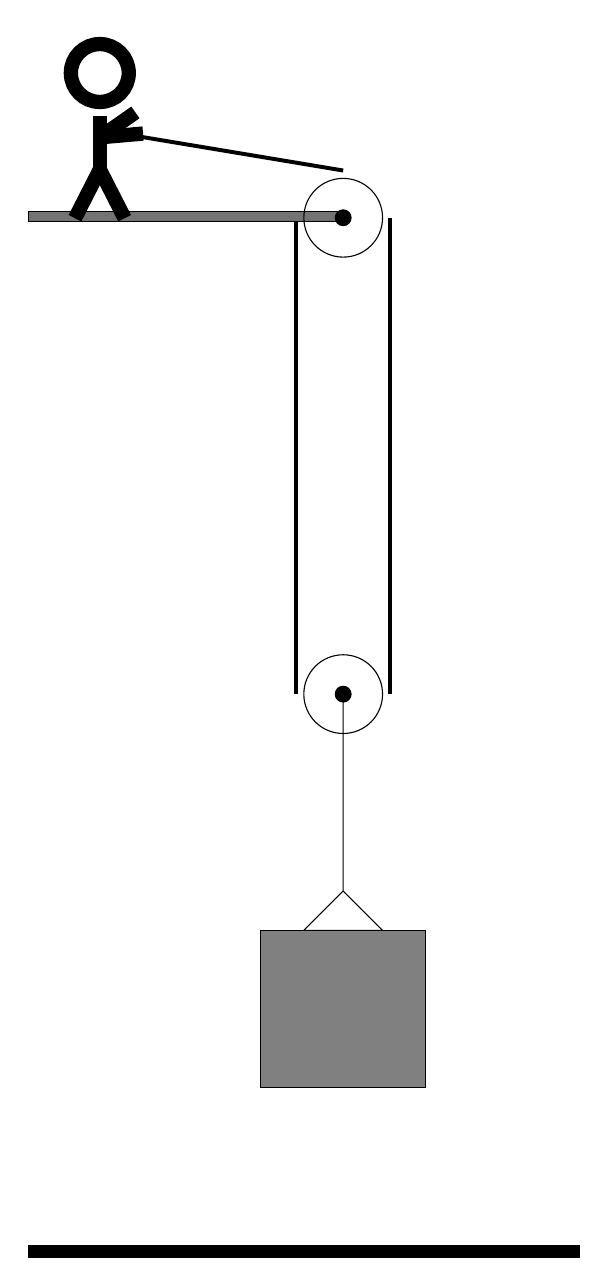
\begin{tikzpicture}
		%%%%% START %%%%%
		\draw[fill=black!55] (-2, 10) rectangle (2, 10.125);
		
		\draw (2, 4.0) circle (0.5);
		\draw[fill=black] (2, 4.0) circle (0.1);
		
		\draw (2, 10.05) circle (0.5);
		\draw[fill=black] (2, 10.05) circle (0.1);
		
		\draw (2, 4.0) -- (2, 1.5) -- (1.5, 1.0) -- (2.5, 1.0) -- (2, 1.5);
		\draw[fill=black!50] (0.95, 1.0) rectangle (3.05, -1.0);
		
		\draw[line width=0.5mm] (1.4, 10) -- (1.4, 4.0);
		\centerarc[line width=0.5mm](2, 4.0)(180:360:0.6);
		\draw[line width=0.5mm](2.6, 4.0) -- (2.6, 10.05);
		\centerarc[line width=0.5mm](2, 10.05)(0:90:0.6);
		\draw[line width=0.5mm](2, 10.65) -- (-1, 11.15);
		
		\node at (-1, 11.15) {\Strichmaxerl[10][-175][35]};
		
		\draw[fill=black] (-2, -3) rectangle (5, -3.15);
		%%%%% END %%%%%
	\end{tikzpicture}
\end{document}